\chapter{Solución}

Una vez nos hemos situado en el contexto en el que se ubica este proyecto, y hemos expuesto los requisitos a cumplir y las herramientas necesarias para llegar a las metas planteadas, nos adentramos a explicar en este capitulo las soluciones utilizadas para llegar a buen puerto.\\

\section{Estructura general}

Como primer problema se presentó decidir cuál de los dos ordenadores que necesitamos para la conexión WebRTC seria el que realizaría la llamada y en que momento del flujo. Este no es un problema trivial, ya que la selección de uno u otro haría que el desarrollo de la aplicación fuese completamente distinto.\\

Se optó por que el par que llevase la batuta de la conexión fuese el ordenador local, ya que este a su vez también es el encargado de  establecer la conexión con el drone. De esta manera tenemos un par que es el que actuará de maestro, estableciendo ambas conexiones en los momentos oportunos.\\

Como ya se comento en la sección \ref{sec:senalizacion} el momento en el que se envía y se recibe cada paquete de información es critico en este sistema de señalización de de oferta/respuesta, por lo que el flujo de la comunicación se diseñó y se ha desarrollado como se muestra en la figura \ref{fig:flujodellamada}.\\


\begin{figure}[htb]
\centering
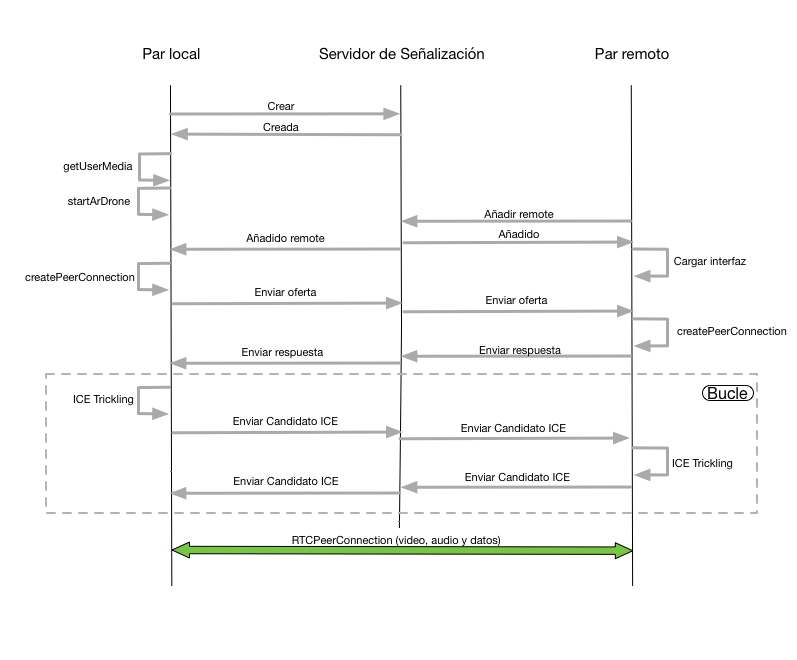
\includegraphics[width=1.1\textwidth]{diagrama_general}
\caption{Flujo de llamada del proyecto}
\label{fig:flujodellamada}
\end{figure}



\section{Señalización}

Las necesidades que que necesitamos cubrir en cuento al servidor de señalización es que sea capaz de intercambiar los datos de red necesarios (Candidatos ICE) y de paquetes SDP. El intercambio debe hacerse con el protocolo de oferta/respuesta según lo establecido en la arquitectura JSEP explicada con anterioridad.\\

Se ha optado por desarrollar el servidor escrito en el lenguaje de programación \emph{Node.js}\footnote{https://nodejs.org/}. Las razones por las que hemos elegido este servidor es que está escrito en JavaScript, por lo que nos resulta muy útil al utilizarse el mismo lenguaje de programación que vamos a utilizar para el resto del proyecto. Por otro lado es un servidor muy liviano.\\

Para cumplir con la arquitectura JSEP vamos a utilizar la librería \emph{Socket.io}\footnote{http://socket.io}, la cuál nos facilita el desarrollo de aplicaciones con necesidades de conexión entre equipos a traves de Websockets.\\

Como se puede ver en la figura anterior, al servidor se le envían 4 tipos de paquetes. Cuando se conecta el par local, cuando se conecta el par remoto, intercambio de candidatos ICE e intercambio de SDP. Sabiendo que tanto los candidatos ICE como los paquetes SDP son objetos, decidimos crear el servidor aceptando tres diferentes tipos de paquetes: el inicial del par local, el inicial del par remoto, y mensajes genéricos que contendrían los objetos anteriormente mencionados. Así pues, esta es la forma del código que gestiona en el servidor el intercambio de paquetes para la señalización.\\

\begin{lstlisting}[caption=Ejemplo paquete SDP]

io.sockets.on('connection', function (socket){

	// Manejaador de mensajes genericos 'message' (intercambios SDP y Candidatos ICE)
	socket.on('message', function (message) {
		//log('Server --> got message: ', message);
		// Si el que envia es Droner hay que mandarlo al remote
		if (socket.id == dronerID) {
			io.sockets.socket(newPeer).emit('message', message);
		// Si el que envia es remote hay que mandarselo al droner
		} else if (socket.id== newPeer) {
			io.sockets.socket(dronerID).emit('message', message);
		} 
	});

	// manejador de mensjes 'create'  enviados por Droner
	socket.on('create', function () {
		//log('Server --> Droner has sido conectado');
		socket.join();
		dronerID = socket.id;
		socket.emit('created');
	});
	

	// Manejador de mensajes 'join remote ' enviados por remote
	socket.on('join remote', function () {
		//log("Server --> Un 'remote' se ha unido.");
		
		io.sockets.in().emit('join remote');
		socket.join();
		newPeer = socket.id;
		socket.emit('joined');
	});
});
\end{lstlisting}


\section{Conexión con la API del drone}

Para establecer la conexión con el drone se ha utilizado el componente \texttt{ardrone\_server} de JdeRobot. Este componente tiene dos versiones, la componente simulada que es la que hemos instalado en forma de plugin en el simulador Gazebo y la componente real, que se conecta al drone real. Ambas componentes nos ofrecen las mismas interfaces de conexión, a las que nos tendremos que conectar.\\

Los componentes JdeRobot utilizan, como ya hemos visto, interfaces ICE para el intercambio de información del que se ocipan. En nuestro caso hemos tenido que instalar el plugin ICE for JavaScrit, o ICE\-JS. Para activar este plugin tenemos que añadir en los archivos de configuración del componente mediante la siguiente linea al comienzo del archivo:\\

\begin{lstlisting}[caption=Activación del plugin ICEJS]
# ICE-JS
Ice.Plugin.IceWS=IceWS:createIceWS
\end{lstlisting}

Posteriormente a esto, en el mismo archivo hay que indicarle las direcciones IP y los puertos a cada interfaz de conexión. Cada conexión se corresponderá con un \emph{WebSocket}, y la nomenclatura es la siguiente:\\

\begin{lstlisting}[caption=Formato \emph{endpoints} de los \emph{WebSocket} de ICEJS]
# ICE-JS
:ws -h ip -p puerto
\end{lstlisting}

Así pues, esta es la forma final que tiene nuestro archivo de configuración:\\

\begin{lstlisting}[caption=Archivo de configuracion]
# Ice-JS
Ice.Plugin.IceWS=IceWS:createIceWS

# Variables de control para ver traceroutes de las conexiones ICE.
#Ice.Trace.Network = 3
#Ice.Trace.Protocol=1


Quadrotor.Control.Endpoints=default -h localhost -p 9850


Quadrotor.CMDVel.Name=ardrone_cmdvel
Quadrotor.CMDVel.Endpoints=default -h localhost -p 9850:ws -h 0.0.0.0 -p 11000


Quadrotor.Conf.Name=Conf
Quadrotor.Conf.Endpoints=default -h localhost -p 9997


Quadrotor.Navdata.Name=ardrone_navdata
Quadrotor.Navdata.Endpoints=default -h localhost -p 9700:ws -h 0.0.0.0 -p 15000


Quadrotor.Extra.Name=ardrone_extra
Quadrotor.Extra.Endpoints=default -h localhost -p 9701:ws -h 0.0.0.0 -p 17000


Quadrotor.Camera.Name=Camera
Quadrotor.Camera.Endpoints=default -h localhost -p 9994


ImuPlugin.Name=ardrone_pose3d
ImuPlugin.Endpoints=default -h localhost -p 9000:ws -h 0.0.0.0 -p 19000
\end{lstlisting}

A parte de los \emph{endpoints} es también importante configurar bien el nombre de cada uno de las interfaces, ya que será necesario para una correcta conexión desde el navegador.\\

\section{Uso WebRTC control drone}
\subsection{Transmisión de la cámara a bordo}
\subsection{Sensores de navegación}
\subsection{Órdenes}
\subsection{Localización espacial del drone}


\section{Interfaz amigable y actual}
\subsection{Visualización de las imágenes}
\subsection{Joysticks}
\subsection{Relojes de navegación}